\documentclass[conference]{IEEEtran}
\usepackage{amsmath}
\usepackage{newtxtext,newtxmath}
\usepackage{graphicx}
\usepackage{booktabs}
\usepackage{textcomp}
\usepackage{url}
\usepackage{balance}

% Allow more full-width floats per page so the many wide diagrams do not
% force early page breaks with half-empty columns.
\setcounter{dbltopnumber}{3}
\renewcommand{\dbltopfraction}{0.92}
\setcounter{topnumber}{4}
\renewcommand{\topfraction}{0.92}
\renewcommand{\textfraction}{0.06}

% Compile:  tectonic IEEE_Final_Research_Paper.tex
% or:       pdflatex IEEE_Final_Research_Paper && bibtex IEEE_Final_Research_Paper
%           && pdflatex IEEE_Final_Research_Paper (twice)

\begin{document}

\title{Personalized Indian Meal Recommendation Using Ingredient-Level Recipe
Features: A Machine Learning Approach}

% Six editable author placeholders. No real identity is claimed: the project
% contains no verified author names, affiliations or addresses.
\author{%
\begin{tabular}{@{}c@{\hspace{0.55cm}}c@{\hspace{0.55cm}}c@{}}
{\normalsize Author One} & {\normalsize Author Two} & {\normalsize Author Three} \\[2pt]
{\footnotesize Dept.\ of Computer Science} & {\footnotesize Dept.\ of Computer Science} & {\footnotesize Dept.\ of Computer Science} \\
{\footnotesize Institution Name} & {\footnotesize Institution Name} & {\footnotesize Institution Name} \\
{\footnotesize City, Country} & {\footnotesize City, Country} & {\footnotesize City, Country} \\
{\footnotesize author1@example.org} & {\footnotesize author2@example.org} & {\footnotesize author3@example.org} \\[9pt]
{\normalsize Author Four} & {\normalsize Author Five} & {\normalsize Author Six} \\[2pt]
{\footnotesize Dept.\ of Computer Science} & {\footnotesize Dept.\ of Computer Science} & {\footnotesize Dept.\ of Computer Science} \\
{\footnotesize Institution Name} & {\footnotesize Institution Name} & {\footnotesize Institution Name} \\
{\footnotesize City, Country} & {\footnotesize City, Country} & {\footnotesize City, Country} \\
{\footnotesize author4@example.org} & {\footnotesize author5@example.org} & {\footnotesize author6@example.org} \\
\end{tabular}}

\maketitle

\begin{abstract}
Dietary tools built for Western food environments transfer poorly to Indian diets,
where dishes combine a dozen ingredients, ingredient names vary by region, and
composition data are incomplete. We report a content-based meal-recommendation pipeline
that couples ingredient-level features with cuisine, course and diet metadata, applies
dietary constraints as hard filters, and derives energy targets from anthropometric
input. The corpus holds 6{,}865 recipes, 90{,}862 parsed ingredient rows and 13{,}049
ingredient names; the composition layer uses IFCT 2017 (528 foods, nine nutrient fields)
and the Indian Nutrient Databank (1{,}014 dishes). With no interaction data, four methods
are compared on 50 held-out queries under a proxy relevance function. The deployed ranker
reaches Precision@5 of 0.996, Recall@5 of 0.0157, Diversity@10 of 0.869, Coverage@20 of
0.234 and 180\,ms per query, yet no method meets the project's recall or coverage
requirement, and clustering is poorly separated (best silhouette 0.047). Code analysis
shows the proxy threshold is exceeded by cuisine, course and diet agreement alone, so
near-ceiling precision measures metadata agreement rather than dietary usefulness. No
ingredient-to-IFCT mapping is approved and only 1.43\,\% of rows carry a resolved mass, so
the nutrition engine abstains rather than estimating.
\end{abstract}

\begin{IEEEkeywords} food recommender systems, content-based recommendation, Indian food composition, ingredient parsing, proxy relevance, nutrition targets, clustering evaluation \end{IEEEkeywords}

\section{Introduction} \label{sec:intro}

Non-communicable diseases dominate the Indian disease burden, and the epidemiological transition has been uneven across states \cite{isdb2017}. Diet is a modifiable risk factor and food recommendation is now a recognisable subfield \cite{trattner2017}.

Three properties of the Indian setting block a direct transfer of existing systems. Dishes are composite: a recipe may list a dozen ingredients in household measures, with preparation states that change the mass eaten. Naming is regional, so one ingredient has several spellings. Nutrient values must come from Indian tables: IFCT 2017 gives laboratory values for 528 key foods \cite{ifct2017} but describes raw foods and is incomplete for several nutrients, while the Indian Nutrient Databank (INDB) adds 1{,}014 composite dishes \cite{indb2024}. Neither supplies a mapping from recipe text to food codes, and that mapping decides whether ingredient-level nutrition can be computed.

Content-based recommendation is the natural starting point because it needs no interaction history: items are described by their own features and compared with a query \cite{pazzani2007}. Recipe recommendation has long used such features, from ingredient co-occurrence networks \cite{teng2012} to ingredient-level models that stay competitive when ratings are sparse \cite{freyne2010}. This paper provides such an account, keeping three questions separate: whether the ranker orders candidates sensibly, whether the list is nutritionally meaningful, and whether either claim was validated against people. We contribute a reproducible pipeline with measured coverage at every stage, a controlled four-method comparison with an analysis of why its proxy cannot support the conclusions its numbers invite, a nutrition engine that abstains at zero approved mappings, and an explicit boundary between what was evaluated and what was not.

\section{Related Work} \label{sec:related}

\emph{Content-based recommendation and text weighting.} Content-based systems represent items by features and rank them against a profile \cite{pazzani2007}, with text weighting descending from TF-IDF \cite{salton1988}. No interaction data are needed; the cost is that relevance is defined by feature overlap, which makes evaluation circular unless an external judgement is introduced. Hybrid designs are the standard remedy \cite{burke2002}.

\emph{Recipe recommendation from ingredients.} Teng \emph{et al.} build ingredient co-occurrence and substitution networks that predict ratings \cite{teng2012}, and Freyne and Berkovsky find ingredient-level features competitive when interaction data are sparse \cite{freyne2010}. Both assume the ingredient list describes the dish reliably; for a scraped corpus that assumption is weaker, which is why parsing yield is reported as a result.

\emph{Health-aware recommendation.} Ge \emph{et al.} score recipes against a user's calorie need \cite{ge2015}; Elsweiler \emph{et al.} show that users misjudge recipe healthiness and that ranking can nudge them towards healthier options \cite{elsweiler2017}. Trattner and Elsweiler name the absence of reliable nutrition data and of appropriate evaluation as recurrent obstacles \cite{trattner2017}. We can rank, but cannot attach a nutrient value to what we rank.

\emph{Composition data, targets and evaluation.} IFCT supplies Indian values \cite{ifct2017} and INDB extends coverage to prepared dishes \cite{indb2024}. Proxy-based offline metrics are common when no judgements exist, but their sensitivity to protocol choices is documented \cite{said2014}, so we treat the proxy as an instrument of known bias; recipe collections are also routinely clustered, with the silhouette \cite{rousseeuw1987} the usual index.

\section{Dataset and Methodology} \label{sec:method}

\subsection{Data resources} \label{sec:data}

Table~\ref{tab:datasets} summarises the resources and Fig.~\ref{fig:arch} shows how they enter the pipeline. The corpus is IndianFoodDatasetX (6{,}871 raw records), reduced to 6{,}865 after removing malformed rows; it carries raw and English ingredient text, timing and serving fields, and cuisine, course and diet labels. Parsing yields 90{,}862 ingredient rows over 13{,}049 distinct names, each with 22 fields including quantity, unit, preparation state and gram weight.

IFCT 2017 contributes 528 foods in 18 groups with nine nutrient fields per 100\,g edible portion: moisture, protein, ash, fat, three fibre fractions, available carbohydrate and energy. Fibre and available carbohydrate are jointly missing for 222 of 528 foods (42.0\,\%), and edible-portion factors exist for only 180 codes (34.1\,\%). INDB contributes 1{,}014 composite dishes in 86 columns and serves as a prepared-dish reference, not a mapping target.

\begin{figure*}[!t] \centering 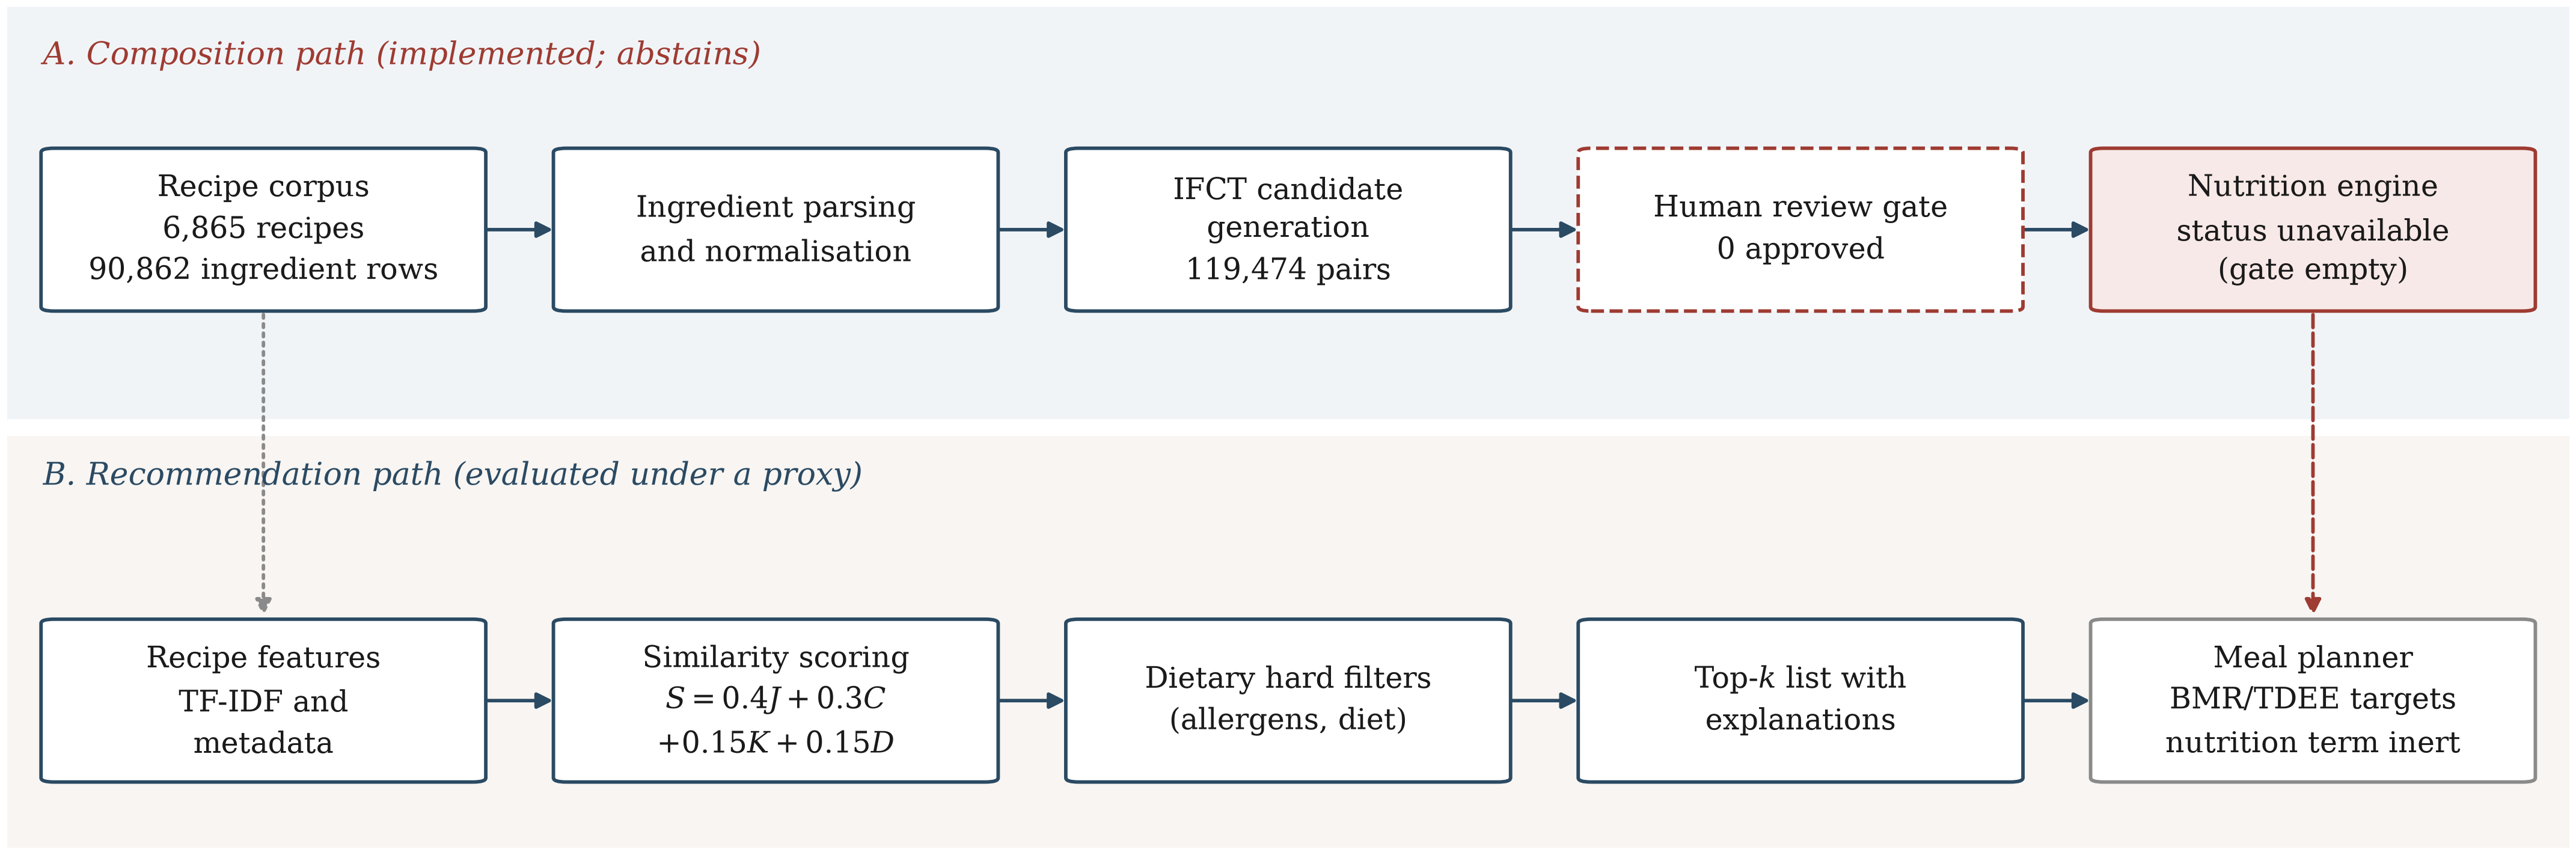
\includegraphics[width=\textwidth]{figures/fig1_architecture.png} \caption{System architecture. Composition (A) parses recipe text, proposes IFCT candidates and requires explicit human approval before any nutrient is computed; the approval store is empty, so the engine returns \texttt{NO\_MAPPED\_INGREDIENTS} and nutrition is shown as unavailable. Recommendation (B) ranks by ingredient overlap and metadata agreement under hard dietary constraints, so it runs without the nutrition layer.} \label{fig:arch} \end{figure*}

% Table I -- data resources. Counts read from data/processed/recipes.parquet,
% data/interim/phase2/parsed_recipe_ingredients.parquet,
% data/interim/ifct_final_candidate/ifct_table1_candidate.parquet,
% data/processed/indb_foods.csv.
\begin{table}[t]
\caption{Data resources and record counts observed in the frozen artifacts.}
\label{tab:datasets}
\centering
\footnotesize
\setlength{\tabcolsep}{3.5pt}
\begin{tabular}{@{}lrp{3.0cm}@{}}
\toprule
\textbf{Resource} & \textbf{Records} & \textbf{Content} \\
\midrule
Recipes       & 6{,}865 & 75 cuisines, 10 courses, 20 diet labels \\
Parsed rows   & 90{,}862 & 13{,}049 names; quantity, unit, state \\
IFCT 2017     & 528 & 18 groups; 9 nutrient fields per 100\,g \\
INDB 2024.11  & 1{,}014 & 86 columns; per-100\,g and per-serving \\
ICMR-NIN 2020 & -- & Reference intakes by age, sex, activity \\
\bottomrule
\end{tabular}
\end{table}


\subsection{Ingredient normalisation and quantity parsing} \label{sec:parsing}

Each ingredient line passes through seven stages: normalisation of case, Unicode and punctuation; synonym mapping to a canonical name; quantity and unit extraction; conversion of household measures to grams; preparation-state extraction; and emission of a structured record. A reconciliation step compares raw and English match results and flags disagreement, recovering rows whose English field was translated inconsistently.

\begin{figure}[!t]
\centering
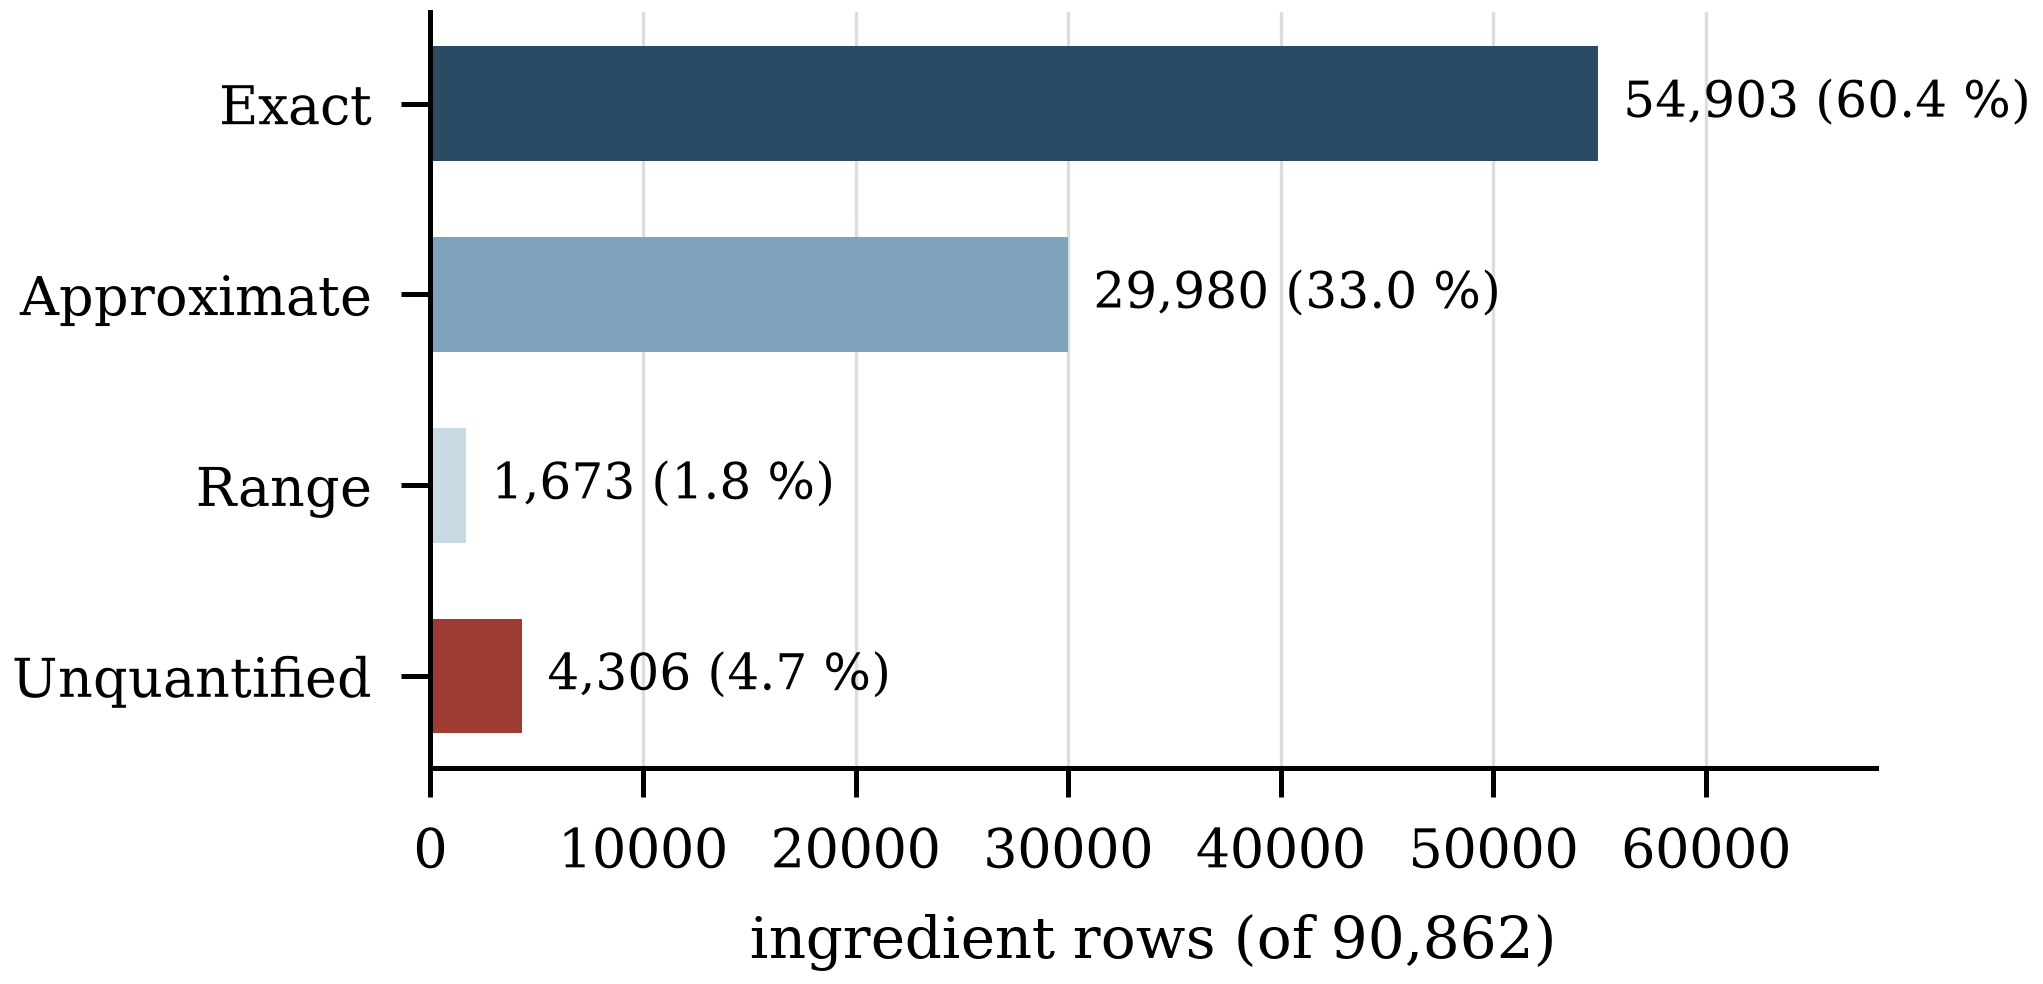
\includegraphics[width=\columnwidth]{figures/fig7_parsing.png}
\caption{Ingredient parsing outcomes over 90{,}862 rows. Exact and approximate parses dominate; unquantified rows carry no mass.}
\label{fig:parsing}
\end{figure}

Table~\ref{tab:preprocessing} and Fig.~\ref{fig:parsing} report the outcome. Of 90{,}862 rows, 54{,}903 (60.4\,\%) parse exactly, 29{,}980 (33.0\,\%) approximately, 1{,}673 (1.8\,\%) as a range and 4{,}306 (4.7\,\%) remain unquantified. A row also needs a convertible unit and a mappable name, and only 1{,}299 rows (1.43\,\%) end with a resolved gram weight. Preparation state is unspecified for 88.6\,\% of rows. Mass coverage is therefore the binding constraint: even perfect mapping would leave over 98\,\% of rows without a mass, and a total computed from the remainder is not a recipe-level total.

% Table II -- preprocessing and quantity-resolution statistics.
% Source: parsed_recipe_ingredients.parquet (parse_status, gram_weight),
% reports/phase3/stage3_6_coverage_analysis.md (preparation state).
\begin{table}[t]
\caption{Ingredient preprocessing statistics over the 90{,}862 parsed rows.
Shares are of the parsed-row total. Only the final row yields a usable mass for
nutrient calculation.}
\label{tab:preprocessing}
\centering
\footnotesize
\setlength{\tabcolsep}{4pt}
\begin{tabular}{@{}lrr@{}}
\toprule
\textbf{Outcome} & \textbf{Rows} & \textbf{Share} \\
\midrule
Exact quantity parsed           & 54{,}903 & 60.4\,\% \\
Approximate quantity parsed     & 29{,}980 & 33.0\,\% \\
Range parsed                    & 1{,}673  & 1.8\,\%  \\
Unquantified                    & 4{,}306  & 4.7\,\%  \\
\midrule
Resolved gram weight            & 1{,}299  & 1.43\,\% \\
Preparation state unspecified   & --       & 88.6\,\% \\
\bottomrule
\end{tabular}
\end{table}


\subsection{Candidate matching and the approval gate} \label{sec:matching}

Normalised names are matched against IFCT food names by string and token similarity, producing 119{,}474 candidate pairs and leaving 63{,}244 rows without a candidate (Fig.~\ref{fig:matching}). A candidate pair is a proposal, not a decision: each must be resolved by a reviewer, and only an approved mapping may enter calculation. The approved-mapping store is currently empty. Candidate counts are sometimes quoted as coverage; they are not, because approval asserts that a composition value is right for the ingredient as used.

\begin{figure*}[!t] \centering 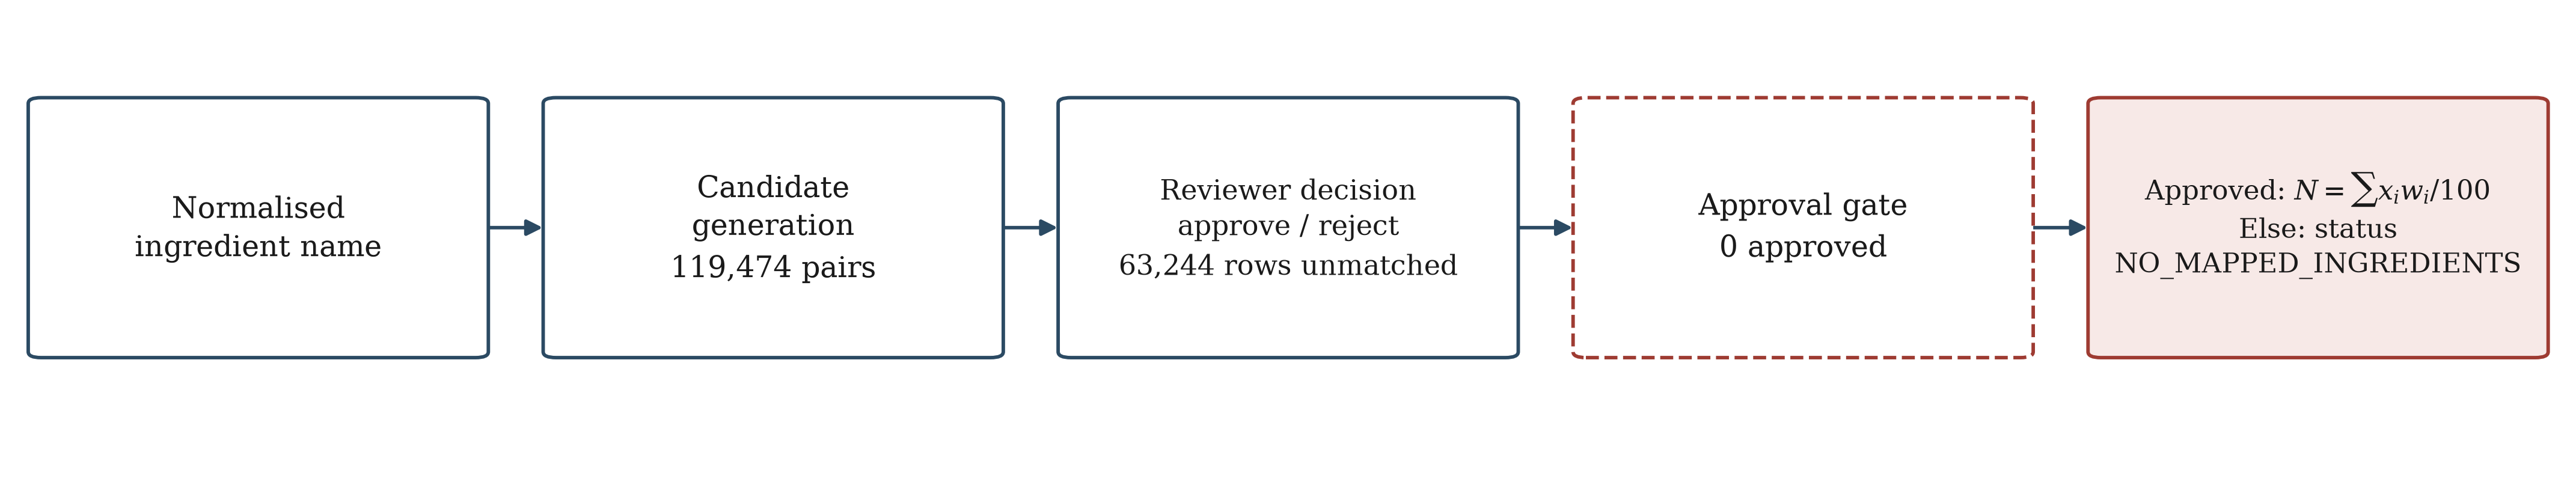
\includegraphics[width=\textwidth]{figures/fig3_matching.png} \caption{Ingredient-to-IFCT matching and nutrition workflow. Candidate generation and reviewer decisions exist; the approval gate is empty, so the only reachable outcome is the unavailable status.} \label{fig:matching} \end{figure*}

\subsection{Nutrient computation and abstention} \label{sec:nutrition}

For an approved mapping with a resolved edible mass the engine computes each nutrient contribution as \begin{equation} \label{eq:nutrient} n_{i} \;=\; \frac{x_{i}\,w_{i}}{100}, \end{equation} where $x_{i}$ is the IFCT value per 100\,g edible portion and $w_{i}$ the edible weight, derived from the parsed mass and the edible-portion factor. Contributions are summed only over rows with both an approved mapping and a known weight, \begin{equation} \label{eq:total} N \;=\; \sum_{i \in \mathcal{A}} n_{i}, \quad \mathcal{A} = \{\, i : \text{mapped}(i) \wedge w_{i} \text{ known} \,\}, \end{equation} a missing nutrient is propagated as absent rather than zero, and per-nutrient completeness $|\mathcal{A}|/|\mathcal{I}|$ accompanies every partial total. With $\mathcal{A}=\varnothing$ every recipe resolves to \texttt{NO\_MAPPED\_INGREDIENTS} and the application shows nutrition as unavailable instead of an estimate. The arithmetic is covered by 42 automated tests with synthetic fixtures, which establish that it computes what it claims, not that its inputs are adequate.

\subsection{Feature representation, ranking and constraints} \label{sec:features}

Each recipe is represented by a TF-IDF vector over its normalised ingredient tokens and by one-hot cuisine, one-hot course and multi-label diet encodings. The vectoriser uses 2{,}000 features, unigrams and bigrams, minimum document frequency 2, maximum document frequency 0.95, sublinear term frequency and L2 normalisation. With term frequency $f_{ij}$, document frequency $n_{j}$ and $N$ recipes in total, each weight is
\begin{equation}
\label{eq:tfidf}
\mathrm{tfidf}_{ij} \;=\; \bigl(1+\log f_{ij}\bigr)\,
\log\bigl(N/n_{j}\bigr)\,\big/\,\lVert \mathbf{t}_{i}\rVert_{2},
\end{equation}
and the representation is fitted on training recipes only.

The deployed ranking function does not consume that matrix: it scores from set overlap and metadata indicators, and the parameter that would enable a TF-IDF path (\texttt{use\_tfidf}) is accepted and then ignored by the method body. It is used by the clustering study but is not a term in \eqref{eq:score}, and the experiment label ``tfidf\_only'' is a misnomer. We report the method by what it computes: \begin{equation} \label{eq:score} S(q,c) \;=\; 0.4\,J(q,c) + 0.3\,C(q,c) + 0.15\,K(q,c) + 0.15\,D(q,c), \end{equation} where $J$ is ingredient Jaccard overlap, $C$ and $K$ are indicator matches on cuisine and course, and $D$ is Jaccard overlap of diet label sets. Dietary constraints -- vegetarian, vegan, eggetarian, Jain, and allergen or ingredient exclusions -- are hard filters applied during candidate traversal, so a constraint-violating recipe is never scored, and self-recommendation is suppressed.

\subsection{Personalisation and meal planning} \label{sec:personal}

The personalisation layer converts a profile into energy and macronutrient targets and uses them to order meal plans. Basal metabolic rate follows Mifflin--St~Jeor \cite{mifflin1990}: \begin{equation} \label{eq:bmr} \mathrm{BMR} = 10\,m + 6.25\,h - 5\,a + s, \quad s = \begin{cases} +5 & \text{male},\\ -161 & \text{female},\end{cases} \end{equation} with mass $m$ in kilograms, height $h$ in centimetres and age $a$ in years. Daily expenditure is $\mathrm{TDEE} = \mathrm{BMR}\cdot \mathrm{PAL}$ with the activity level chosen from ICMR-NIN bands \cite{icmrnin2020}, and the energy target moves by $\pm 500$\,kcal for weight goals; protein, fat and fibre targets follow the same reference. Daily plans assign recipes to meal slots under the dietary filters; weekly plans repeat this.

Two qualifications apply: the targets are arithmetic on self-reported input, never checked against measured expenditure, and because nutrition values are unavailable the planner's nutrition term is inert, so it reduces to similarity plus metadata agreement.

\section{Experimental Setup} \label{sec:setup}

\emph{Environment.} Experiments ran on one Windows machine, CPU only, with Python 3.15.2, scikit-learn 1.9.1, NumPy 2.5.4, pandas 3.1.1 and SciPy 1.18.1.

\emph{Splits.} Recipes are split 70/15/15, stratified by cuisine, seed 42, minimum five recipes per stratum. Smaller categories are dropped, yielding 4{,}783 training, 1{,}025 validation and 1{,}025 test recipes (69.7, 14.9 and 14.9\,\% of 6{,}865; 32 recipes fall outside the strata) over 63 cuisines at recipe level, with zero identifier overlap and zero near-duplicate pairs at ingredient Jaccard $\geq 0.9$ across splits. The evaluation sample is the first 50 test recipes.

\emph{Methods.} Four rankers share the query set, the pool of 6{,}865 recipes and exclusion of the query. \emph{Random} shuffles candidates with seed 42. \emph{Cuisine match} scores $0.6\,C' + 0.4\,J$, where $C'$ gives full credit for an identical cuisine and half credit for cuisines mapping to the same region. \emph{Jaccard} orders by ingredient overlap and drops zero-overlap items. \emph{Weighted} is \eqref{eq:score}.

\emph{Metrics.} For the list $L_q$ of length $k$ and the proxy-relevant set $R_q$, \begin{align} P@k &= \frac{1}{|Q|}\sum_{q\in Q}\frac{|L_q \cap R_q|}{k}, \label{eq:p}\\ R@k &= \frac{1}{|Q|}\sum_{q\in Q}\frac{|L_q \cap R_q|}{|R_q|}, \label{eq:r} \end{align} with $|Q|=50$. Diversity is one minus mean pairwise ingredient Jaccard within the top-10 list, and coverage is the fraction of the catalogue appearing in any list: \begin{align} \mathrm{Div}@k &= 1 - \frac{2}{k(k-1)}\sum_{i<j} J(d_i,d_j), \label{eq:div}\\ \mathrm{Cov}@k &= \Bigl|\bigcup_{q\in Q} L_q\Bigr| \big/ |\mathcal{C}|. \label{eq:cov} \end{align} Coverage is computed over the first 100 catalogue recipes, each contributing a top-20 list, not over the 50 queries; we flag the mismatch.

\emph{Proxy relevance.} With no interaction data and no human judgements, relevance must be defined. A candidate is relevant when
\begin{equation}
\label{eq:proxy}
\rho = 0.5\,J + 0.2\,C + 0.15\,K + 0.15\,D \;\geq\; 0.3,
\end{equation}
where $J$ is ingredient Jaccard overlap and $C$, $K$, $D$ are cuisine, course and diet agreement; $D$ is the overlap coefficient in the evaluation module, although \eqref{eq:score} uses Jaccard for that term. Equation~\eqref{eq:proxy} reuses the quantities the rankers optimise, so it is circular by construction, and permissive: a candidate agreeing on cuisine, course and diet but sharing no ingredient scores $0.5 \geq 0.3$ and is relevant.

\emph{Composite score and requirements.} The project defined four requirements --- $P@5 \geq 0.20$, $R@5 > 0.02$, $\mathrm{Cov}@20 > 0.50$, latency below 500\,ms --- and a composite
\begin{equation}
\label{eq:composite}
\begin{split}
\Phi = {}&0.30P + 0.20R + 0.15\,\mathrm{Div} + 0.15\,\mathrm{Cov}\\
&+ 0.10\left(1-L/500\right) + 0.10\,\mathrm{Rel}.
\end{split}
\end{equation}
The reliability term $\mathrm{Rel}$ was never defined or measured and is set to 1.0 for every method, so it adds a constant and cannot affect the ordering. We report $\Phi$ recomputed with measured inputs; excluding $\mathrm{Rel}$ subtracts 0.10 from every value and leaves the ranking unchanged.

\section{Results and Discussion}
\label{sec:results}

\subsection{Recommendation quality, diversity and coverage}
\label{sec:recresults}

Table~\ref{tab:results} and Fig.~\ref{fig:comparison} report the comparison. The weighted ranker attains the highest precision and proxy recall, the second-highest diversity, coverage of 0.234 and 180\,ms per query. Cuisine match is the strongest baseline and the only method whose precision decays visibly with $k$, because its one-cuisine restriction weakens. Random reaches 0.128, the first sign that the relevant set is large.

\begin{figure*}[!t]
\centering
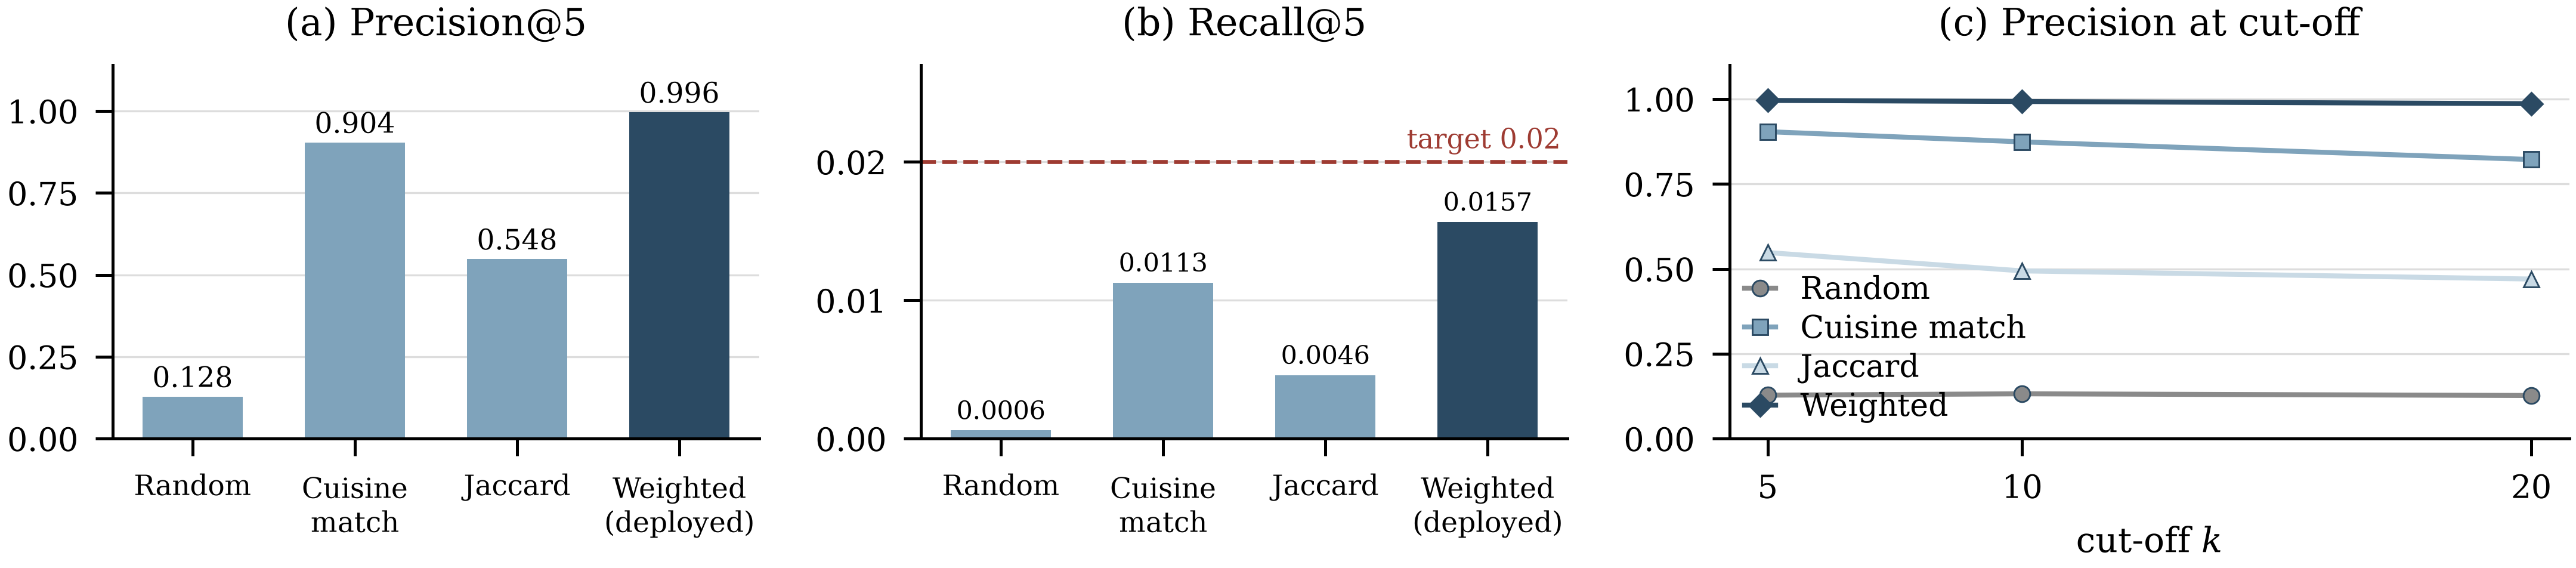
\includegraphics[width=\textwidth]{figures/fig5_comparison.png}
\caption{Performance on the shared 50-query sample: (a) Precision@5; (b) Recall@5 against
the 0.02 requirement, met by no method; (c) precision versus cut-off.}
\label{fig:comparison}
\end{figure*}

% Table III -- recommendation results.
% Sources: baseline_experiments.json, content_based_experiments.json.
% Latency = time_seconds / 50 queries; composite recomputed from the project
% formula with Rel = 1 for every method (see Section IV-E).
\begin{table}[t]
\caption{Recommendation results on the same 50 held-out queries and the same
6{,}865-recipe candidate pool. Latency is mean wall-clock time per query.
$\Phi$ is the project's composite score; its constant reliability term makes it a
bookkeeping device, not a validated utility.}
\label{tab:results}
\centering
\scriptsize
\setlength{\tabcolsep}{3.4pt}
\begin{tabular}{@{}lcccccc@{}}
\toprule
\textbf{Method} & \textbf{P@5} & \textbf{R@5} & \textbf{Div@10} & \textbf{Cov@20} & \textbf{Lat. (ms)} & \textbf{$\Phi$} \\
\midrule
Random            & 0.128 & 0.0006 & 0.958 & 0.254 & 110 & 0.398 \\
Cuisine match     & 0.904 & 0.0113 & 0.824 & 0.225 & 390 & 0.553 \\
Jaccard           & 0.548 & 0.0046 & 0.773 & 0.220 & 208 & 0.473 \\
Weighted (deployed) & \textbf{0.996} & \textbf{0.0157} & 0.869 & 0.234 & 180 & \textbf{0.631} \\
\bottomrule
\end{tabular}
\end{table}


Precision@5 near unity means almost every returned recipe clears the proxy threshold; it does not mean the recipes are useful. Recall is structurally low because five results cover only a fraction of a large relevant set: the two metrics bound that set, since $|R_q| = k\,P@k/R@k$, giving about 317 relevant items per query and a maximum attainable Recall@5 near 1.6\,\%. The composite is driven almost entirely by its precision term.

\begin{figure*}[!t]
\centering
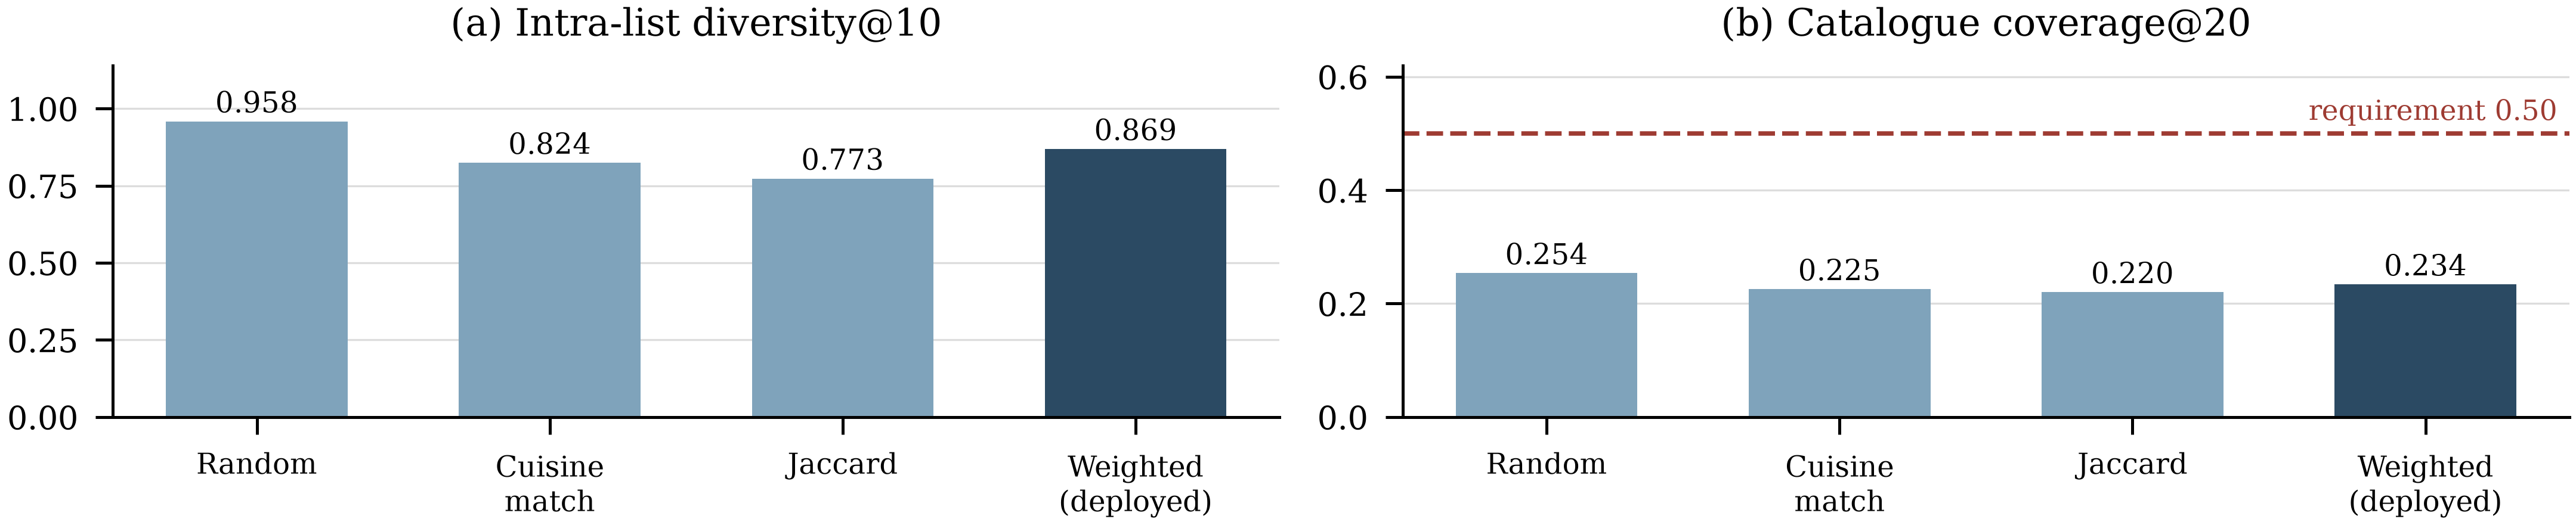
\includegraphics[width=\textwidth]{figures/fig6_divcov.png}
\caption{Intra-list diversity@10 (a) and catalogue coverage@20 (b) with the requirement
marked. Every method falls short by at least a factor of two.}
\label{fig:divcov}
\end{figure*}

Fig.~\ref{fig:divcov} shows the resulting trade-off: coverage is maximal for random and lowest for Jaccard, every value is below half the 0.50 requirement, and diversity runs the other way. Only the weighted ranker meets the precision and latency requirements; its recall and coverage failures are recorded rather than waived.

\subsection{Why the proxy flatters the rankers}
\label{sec:bias}

Equation~\eqref{eq:proxy} gives half its weight to ingredient Jaccard and the rest to metadata agreement, but its threshold is 0.3 --- below the 0.5 that metadata agreement alone supplies. A candidate from the same cuisine, course and diet group is therefore relevant even with no shared ingredient, so the relevant set is dominated by such candidates. This explains the combination of near-ceiling precision and negligible recall: the rankers sample from a large set the proxy has already declared good, as the cuisine baseline's 0.904 shows.

The error analysis corroborates this: across 20 inspected queries, 47 recommended items crossed a cuisine boundary and 16 queries contained generic terms (salt, oil, water, pepper) that the proxy rewards.

\subsection{Clustering}
\label{sec:clustering}

Table~\ref{tab:clustering} and Fig.~\ref{fig:clustering} report clustering on the combined feature matrix reduced to 20 principal components. Both indices indicate weak structure, and a silhouette below 0.05 means the average item is almost as close to a neighbouring cluster as to its own \cite{rousseeuw1987}. Agglomerative clustering is worse on both indices at every $K$, and cluster sizes are skewed (at $K=50$: 287, 3 and 5 recipes). Composition is dominated by cuisine metadata rather than ingredient patterns, so clustering is unsuitable as a primary mechanism; at most it could filter candidates, which we did not evaluate.

% Table IV -- clustering results.
% Source: reports/phase5/experiments/results/clustering_experiments.json
\begin{table}[t]
\caption{Clustering on the combined feature matrix reduced to 20 principal
components (seed 42). Every silhouette is below 0.05 and every Davies--Bouldin
index above 3, i.e.\ no configuration produces well-separated clusters.}
\label{tab:clustering}
\centering
\footnotesize
\setlength{\tabcolsep}{4pt}
\begin{tabular}{@{}llccc@{}}
\toprule
\textbf{Algorithm} & \textbf{$K$} & \textbf{Silhouette} & \textbf{Davies--Bouldin} & \textbf{Largest} \\
\midrule
K-Means       & 20  & 0.0388 & 4.111 & 655 \\
K-Means       & 50  & \textbf{0.0469} & 3.603 & 287 \\
K-Means       & 100 & 0.0414 & \textbf{3.187} & 201 \\
Agglomerative & 20  & 0.0172 & 4.214 & 1{,}516 \\
Agglomerative & 50  & 0.0244 & 3.605 & 613 \\
\bottomrule
\end{tabular}
\end{table}


\begin{figure}[!t]
\centering
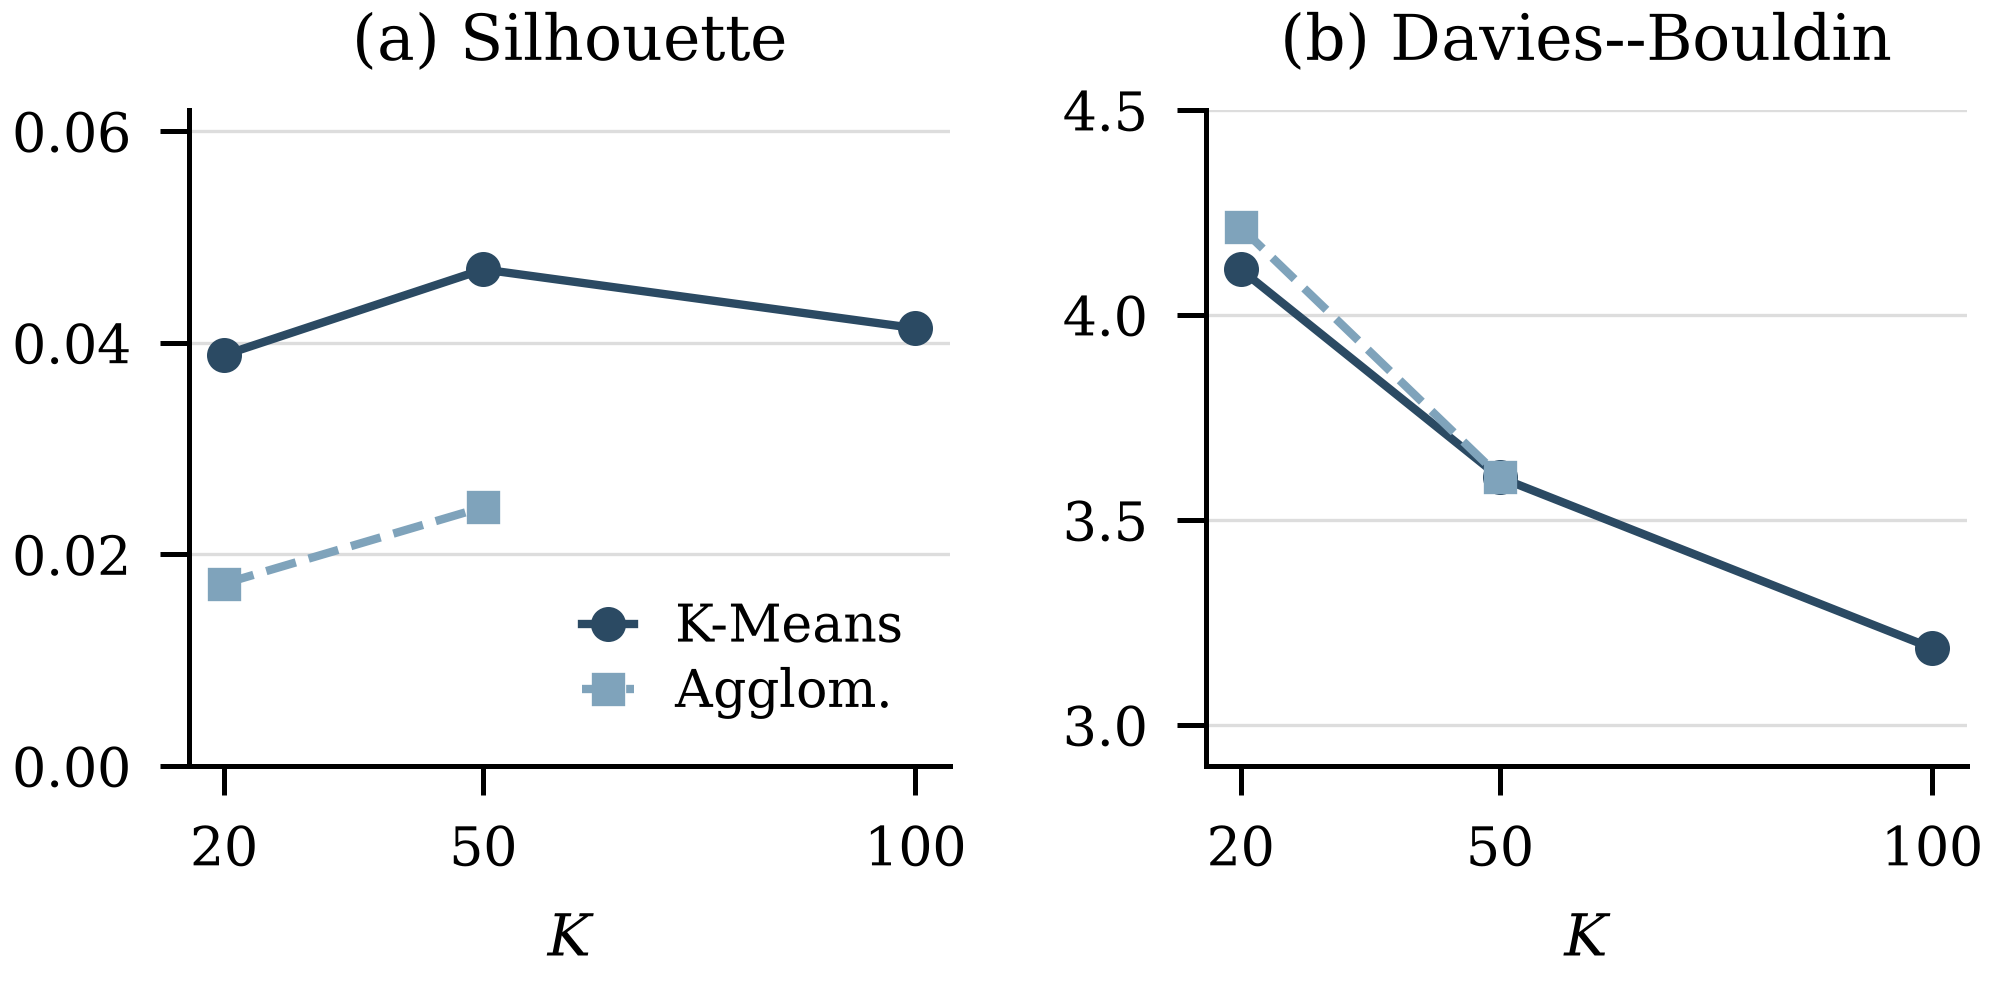
\includegraphics[width=\columnwidth]{figures/fig9_clustering.png}
\caption{Clustering diagnostics versus $K$. Silhouette (a) never exceeds 0.05 and
Davies--Bouldin (b) never falls below 3.}
\label{fig:clustering}
\end{figure}

\subsection{The nutrition pipeline}
\label{sec:nutrresults}

Fig.~\ref{fig:nutrition} summarises the composition path: zero approved mappings, 1.43\,\% of rows with a resolved mass, edible-portion factors for 34.1\,\% of IFCT codes, and fibre plus available carbohydrate present for 306 of 528 foods (58.0\,\%). Preparation state is unspecified for 88.6\,\% of rows, and IFCT describes raw foods while recipes describe cooked dishes. The engine's abstention is specified and tested, and the application shows an unavailable status rather than zeros --- a system reporting neither partial sums nor imputed values is more useful to a dietitian than one reporting a confident wrong number.

\begin{figure}[!t]
\centering
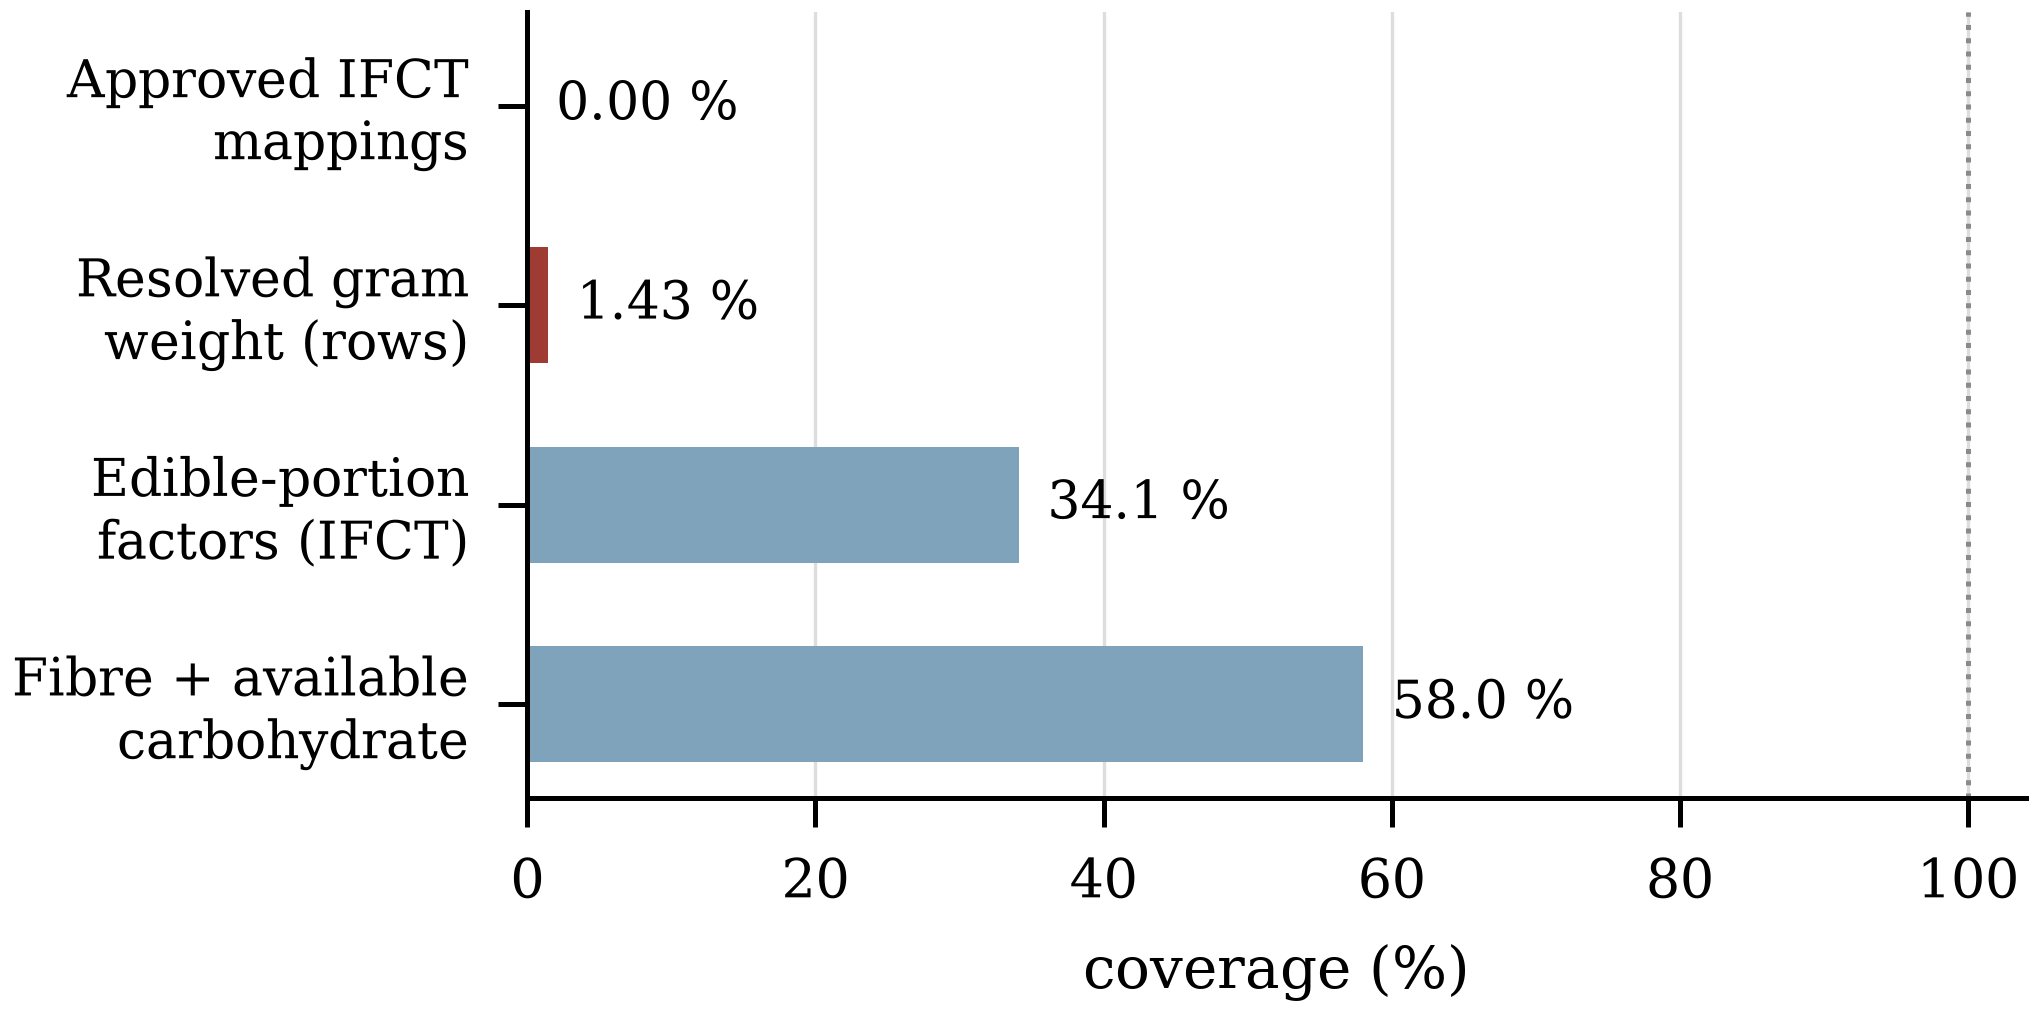
\includegraphics[width=\columnwidth]{figures/fig8_nutrition.png}
\caption{Measured coverage of the four inputs the engine needs. The first two bars are measured
on recipe rows, the last two on IFCT records.}
\label{fig:nutrition}
\end{figure}

\subsection{Configuration defect and composite limitation}
\label{sec:defect}

The content-based experiments ran under four nominal weight configurations, and all four
produced numerically identical metrics. Inspection of the retrieval code shows why: the ranker
hard-codes the weights of \eqref{eq:score}, and never reads the configuration object. The agreement is a software defect, not evidence that the weights are insensitive, so we report a single configuration and withdraw the sensitivity claim.

The composite has a separate defect: its reliability term was never defined, so it contributes a
constant 0.10 to every method and cannot discriminate between them. We report $\Phi$ as bookkeeping, not validated utility; the earlier summary's composites are not reproducible from \eqref{eq:composite}.

\subsection{Discussion and limitations}
\label{sec:limits}

The evaluation is bounded. It uses 50 queries from one corpus, drawn as the first 50 test recipes rather than at random, with a proxy sharing features with the models it scores, so it supports comparisons among these methods only and cannot establish that ingredient modelling helps. No human judgements, user study or clinical assessment were performed, and the absence of interaction data rules out collaborative filtering. The corpus is scraped, carries no explicit licence and mixes regional naming conventions. Nutrient accuracy is untested for the same reason the engine abstains, the target arithmetic inherits the assumptions of \cite{mifflin1990} and \cite{icmrnin2020} without validation against measured expenditure.

\section{Conclusion}
\label{sec:conclusion}

We rebuilt and evaluated a content-based pipeline for personalised Indian meal recommendation
that combines ingredient-level set features with cuisine, course and diet metadata, applies
dietary constraints as hard filters, and derives energy and macronutrient targets from
anthropometry and Indian reference intakes. On 50 held-out queries the deployed ranker reaches
Precision@5 of 0.996, Recall@5 of 0.0157, Diversity@10 of 0.869, Coverage@20 of 0.234 and
180\,ms per query, and it nevertheless fails the
project's recall and coverage requirements, as does every other method, and clustering offers no
usable structure (best silhouette 0.047).

Two findings matter more than the ranking numbers. The relevance proxy can be satisfied by metadata agreement alone, so near-ceiling precision measures agreement between labels rather than the usefulness of a meal; and the composition component cannot be validated in its current state, because no ingredient-to-IFCT mapping is approved and 1.43\,\% of rows carry a resolved mass. The honest summary is a working ranking component, evaluated under a biased proxy, attached to an implemented, tested and deliberately silent nutrition component. Closing that gap is as much curation as algorithm design: approve mappings for frequent ingredients, extend mass coverage, record preparation states, and collect genuine relevance judgements.

\balance
\bibliographystyle{IEEEtran}
\bibliography{references}

\end{document}
